\documentclass[a4paper, 12pt]{article}
\usepackage[a4paper,top=1.5cm, bottom=1.5cm, left=1cm, right=1cm]{geometry}

% Работа с русским языком
\usepackage[utf8]{inputenc}
\usepackage{mathtext}                % русские буквы в формулах
\usepackage[english, russian]{babel} % локализация и переносы

\usepackage{graphicx}   % Вставка изображений
\usepackage{float}      % "Плавающие" изображения3
\usepackage{wrapfig}    % Обтекание фигур (таблиц, картинок и прочего)
\graphicspath{ {./images/} }

\usepackage{tabularx}
\usepackage{multirow}
\usepackage{amsmath}
\usepackage{amsfonts}
\usepackage{indentfirst}
\usepackage{longtable}
\graphicspath{{pictures/}}
\usepackage{natbib}

%%% Колонтитулы
\usepackage{titleps}
\newpagestyle{main}{
	\setheadrule{0.4pt}
	\sethead{Отчёт о выполнении лабораторной работы 2.1.6}{}{}
	\setfootrule{0.4pt}                       
	\setfoot{ФРКТ МФТИ, 2023}{}{\thepage} 
}
\pagestyle{main}  

\begin{document}
    \begin{titlepage}
	\begin{center}
            {\large МОСКОВСКИЙ ФИЗИКО-ТЕХНИЧЕСКИЙ ИНСТИТУТ (НАЦИОНАЛЬНЫЙ       ИССЛЕДОВАТЕЛЬСКИЙ УНИВЕРСИТЕТ)}
	\end{center}
 
	\begin{center}
		{\large Физтех-школа радиотехники и компьютерных технологий}
	\end{center}
	
	\vspace{8cm}
	{\LARGE
		\begin{center}
                {\bf Отчёт о выполнении лабораторной работы 2.1.6}\\
                Эффект Джоуля-Томсона
		\end{center}
	}
	\vspace{5cm}
	\begin{flushright}
		{\Large Автор:\\ Тихонов Дмитрий Романович, \\
			\vspace{0.2cm}
			студент группы Б01-206}
	\end{flushright}
	\vspace{5cm}
	\begin{center}
		\Large Долгопрудный, 2023
	\end{center}
    \end{titlepage}

    \section*{Введение}

    \noindent \textbf{Цель работы:}  
    \begin{enumerate}
        \item определение изменения температуры углекислого газа при протекании через малопроницаемую перегородку при разных начальных значениях давления и температуры;
        \item вычисление по результатам опытов коэффициентов Ван-дер-Ваальса $a$ и $b$.
    \end{enumerate}

    \noindent \textbf{В работе используются:} трубка с пористой перегородкой; труба Дьюара; термостат; термометры; дифференциальная термопара; микровольтметр; балластный баллон; манометр.
    
    \section*{Теоретические сведения}

    \noindent Эффектом Джоуля–Томсона называется изменение температуры газа, медленно протекающего из области высокого в область низкого давления в условиях хорошей тепловой изоляции. В разреженных газах, которые приближаются по своим свойствам к идеальному газу, при таком течении температура газа не меняется. Эффект Джоуля–Томсона демонстрирует отличие исследуемого газа от идеального.\\

    \noindent В работе исследуется изменение температуры углекислого газа при медленном его течении по трубке с пористой перегородкой (риc. \ref{ust}). Трубка 1 хорошо теплоизолирована. Газ из области повышенного давления $P_1$ проходит через множество узких и длинных каналов пористой перегородки 2 в область с атмосферным давлением $P_2$. Перепад давления $\Delta P = P_1 - P_2$ из-за большого сопротивления каналов может быть заметным даже при малой скорости течения газа в трубке. Величина эффекта Джоуля–Томсона определяется по разности температуры газа до и после перегородки.\\

    \noindent Рассмотрим стационарный поток газа между произвольными сечениями I и II трубки (до перегородки и после нее). Пусть, для определенности, через трубку прошел 1 моль углекислого газа; $\mu$ -- его молярная масса. Молярные объемы газа, его давления и отнесенные к молю внутренние энергии газа в сечениях I и II обозначим соответственно $V_1, P_1, U_1 $ и $ V_2, P_2, U_2$. Для того чтобы ввести в трубку объем $V_1$, над газом нужно совершить работу $A_1 = P_1V_1$. Проходя через сечение II, газ сам совершает работу $A_2 = P_2V_2$. Так как через боковые стенки не происходит ни обмена теплом, ни передачи механической энергии, то

    \begin{equation}
        \label{1}
        A_1-A_2=\left(U_2+\frac{\mu v_2^2}{2}\right) - \left(U_1 + \frac{\mu v_1^2}{2}\right).
    \end{equation}

    \noindent В уравнении \eqref{1} учтено изменение как внутренней (первые члены в скобках), так и кинетической (вторые члены в скобках) энергии газа. Подставляя в \eqref{1} написанные выражения для $A_1$ и $A_2$ и перегруппировывая члены, найдем

    \begin{equation}
        \label{2}
        H_1-H_2=\left(U_1+P_1V_1\right) - \left(U_2 + P_2V_2\right) = \frac{1}{2} \mu \left(v^2_2-v^2_1\right).
    \end{equation}

    \noindent Сделаем несколько замечаний. Прежде всего отметим, что в процессе Джоуля–Томсона газ испытывает в пористой перегородке существенное трение, приводящее к ее нагреву. Потери энергии на нагрев трубки в начале процесса могут быть очень существенными и сильно искажают ход явления. После того как температура трубки установится и газ станет уносить с собой все выделенное им в пробке тепло, формула \eqref{1} становится точной, если, конечно, теплоизоляция трубки достаточно хороша и не происходит утечек тепла наружу через ее стенки.\\

    \noindent Второе замечание связано с правой частью \eqref{2}. Процесс Джоуля–Томсона в чистом виде осуществляется лишь в том случае, если правой частью можно пренебречь, т. е. если макроскопическая скорость газа с обеих сторон трубки достаточно мала. У нас сейчас нет критерия, который позволил бы установить, когда это можно сделать. В силу сохранения энтропии в случае реального газа получаем:

    \begin{equation}
        \label{3}
        \mu_\text{Д--Т} = \frac{\Delta T}{\Delta P} \approx \frac{(2a/RT) - b}{C_P}.
    \end{equation}

    \noindent Из формулы \eqref{3} видно, что эффект Джоуля–Томсона для не очень плотного газа зависит от соотношения величин $a$ и $b$, которые оказывают противоположное влияние на знак эффекта. Если силы взаимодействия между молекулами велики, так что превалирует <<поправка на давление>>, то основную роль играет член, содержащий $a$, и \[ \frac{\Delta T}{\Delta P} > 0, \] т. е. газ при расширении охлаждается ($\Delta T < 0$, так как всегда $\Delta P < 0 $). В другом случае \[ \frac{\Delta T}{\Delta P} < 0, \] т. е. газ нагревается ($ \Delta T > 0 $, так как по-прежнему $ \Delta P < 0 $).\\

    \noindent Этот результат нетрудно понять из энергетических соображений. Как мы уже знаем, у идеального газа эффект Джоуля–Томсона отсутствует. Идеальный газ отличается от реального тем, что в нем можно пренебречь потенциальной энергией взаимодействия молекул. Наличие этой энергии приводит к охлаждению или нагреванию реальных газов при расширении. При больших $a$ велика энергия притяжения молекул. Это означает, что потенциальная энергия молекул при их сближении уменьшается, а при удалении -- при расширении газа -- возрастает. Возрастание потенциальной энергии молекул происходит за счет их кинетической энергии -- температура газа при расширении падает. Аналогичные рассуждения позволяют понять, почему расширяющийся газ нагревается при больших значениях $b$.\\

    \noindent Как следует из формулы \eqref{3}, при температуре \[ T_i = \frac{2a}{Rb} \] коэффициент $\mu_\text{Д--Т}$ обращается в нуль. По формулам связи параметров газа Ван-дер-Ваальса с критическими параметрами получаем: 

    \begin{equation}
        \label{4}
        T_\text{инв} = \frac{27}{4} T_\text{кр}.
    \end{equation}

    \noindent При температуре $T_\text{инв}$ эффект Джоуля–Томсона меняет знак: ниже температуры инверсии эффект положителен ($\mu_\text{Д--Т} > 0$, газ охлаждается), выше $T_\text{инв}$ эффект отрицателен ($\mu_\text{Д--Т} < 0$, газ нагревается).\\

    \noindent Вернемся к влиянию правой части уравнения \eqref{2} на изменение температуры расширяющегося газа. Для этого сравним изменение температуры, происходящее вследствие эффекта Джоуля–Томсона, с изменением температуры, возникающим из-за изменения кинетической энергии газа. Увеличение кинетической энергии газа вызывает заметное и приблизительно одинаковое понижение его температуры как у реальных, так и у идеальных газов. Поэтому при оценках нет смысла пользоваться сложными формулами для газа Ван-дер-Ваальса.\\

    \noindent Заменяя в формуле \eqref{2} $U$ через $C_VT$ и $PV$ через $RT$, найдем \[ \left(R+C_V\right)\left(T_1-T_2\right)=\mu\left(v_2^2-v_1^2\right)/2 \] или \[ \Delta T = \frac{\mu}{2C_P}\left(v_2^2-v_1^2\right). \]
    
    \noindent В условиях нашего опыта расход газа $Q$ на выходе из пористой перегородки не превышает $10 $ см$ ^3 $/с, а диаметр трубки равен 3 мм. Поэтому \[ v_2<=\frac{4Q}{\pi d^2} = \frac{4 \text{ см}^3/\text{с}}{3,14\cdot(0,3)^2\text{ см}^2} \approx 140 \text{ см}/\text{с}. \]

    \noindent Скорость $v_1$ газа у входа в пробку относится к скорости $v_2$ у выхода из нее как давление $P_2$ относится к $P_1$. В нашей установке $P_1 = 4$ атм, a $P_2 = 1$ атм, поэтому \[ v_1=\frac{P_2}{P_1}v_2 = 35 \text{ см}/\text{с}. \]Для углекислого газа $ \mu = 44 $ г/моль, $ C_P = 40 $ Дж/(моль·К), имеем \[ \Delta T = \frac{\mu}{2C_P}\left(v_2^2-v_1^2\right) \approx 7\cdot10^{-4} \text{ K}. \]

    \noindent Это изменение температуры ничтожно мало по сравнению с измеряемым эффектом (несколько градусов).\\

    \noindent В данной лабораторной работе исследуется коэффициент дифференциального эффекта Джоуля–Томсона для углекислого газа. По экспериментальным результатам оценивается коэффициент теплового расширения, постоянные в уравнении Ван-дер-Ваальса и температура инверсии углекислого газа. Начальная температура газа $T_1$ задается термостатом. Измерения проводятся при трех температурах: комнатной, 30 $ ^\circ $C и 50 $^\circ $C.

    \section*{Методика измерений и используемое оборудование}

    \begin{figure}[H]
        \centering
        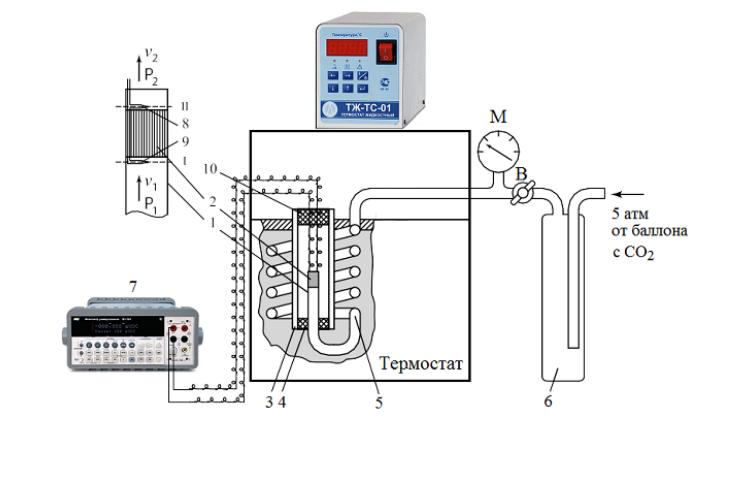
\includegraphics[width=18cm]{images/installation.png}
        \caption{Экспериментальная установка}
        \label{ust}
    \end{figure}
    
    \noindent Схема установки для исследования эффекта Джоуля–Томсона в углекислом газе представлена на рисунке \ref{ust}. Основным элементом установки является трубка 1 с пористой перегородкой 2, через которую пропускается исследуемый газ. Трубка имеет длину 80 мм и сделана из нержавеющей стали, обладающей, как известно, малой теплопроводностью. Диаметр трубки $d = 3$~мм, толщина стенок 0,2 мм. Пористая перегородка расположена в конце трубки и представляет собой стеклянную пористую пробку со множеством узких и длинных каналов. Пористость и толщина пробки ($l = 5$ мм) подобраны так, чтобы обеспечить оптимальный поток газа при перепаде давлений $\Delta P = 4$ атм (расход газа составляет около $10$ см$^3$/с); при этом в результате эффекта Джоуля–Томсона создается достаточная разность температур.\\

    \noindent Углекислый газ под повышенным давлением поступает в трубку через змеевик 5 из балластного баллона 6. Медный змеевик омывается водой и нагревает медленно протекающий через него газ до температуры воды в термостате. Температура воды измеряется термометром, помещенным в термостате. Термостат снабжён автоматическим терморегулятором, поддерживающим постоянной температуру воды в нём сточностью $\pm 0,1 ^\circ$C.\\
    
    \noindent Давление газа в трубке измеряется манометром М и регулируется вентилем В (при открывании вентиля В, т. е. при повороте ручки против часовой стрелки, давление $ P_1 $ повышается). Манометр М измеряет разность между давлением внутри трубки и наружным (атмосферным) давлением. Так как углекислый газ после пористой перегородки выходит в область с атмосферным давлением $P_2$, то этот манометр непосредственно измеряет перепад давления на входе и на выходе трубки $\Delta P = P_1 - P_2 $.\\

    \noindent Разность температур газа до перегородки и после нее измеряется дифференциальной термопарой медь -- константан. Константановая проволока диаметром 0,1 мм соединяет спаи 8 и 9, а медные проволоки (того же диаметра) подсоединены к цифровому вольтметру 7. Отвод тепла через проволоку столь малого сечения пренебрежимо мал. Для уменьшения теплоотвода трубка с пористой перегородкой помещена в трубу Дьюара 3, стенки которой посеребрены, для уменьшения теплоотдачи, связанной с излучением. Для уменьшения теплоотдачи за счет конвекции один конец трубы Дьюара уплотнен кольцом 4, а другой закрыт пробкой 10 из пенопласта. Такая пробка практически не создает перепада давлений между внутренней полостью трубы и атмосферой.

    \section*{Результаты измерений и обработка данных}

    \subsection*{Определение коэффициента Джоуля-Томсона}

    \noindent Проведём измерение зависимости $\Delta T$ от $\Delta P$ для разных значений температур. Полученные значения заносим в таблицы \ref{tab:25C}, \ref{tab:35C}, \ref{tab:45C} и \ref{tab:55C}. При записи полученных данных также учитываем, что чувствительность термопары медь -- константан зависит от температуры. При вычислении будем использовать следующую формулу: \[ \Delta T = \frac{U}{\alpha}, \] где $\alpha_{25^\circ C} = 40,7 \text{ мкВ}/^\circ C$, $\alpha_{35^\circ C} = 41,5 \text{ мкВ}/^\circ C$, $\alpha_{45^\circ C} = 42,4 \text{ мкВ}/^\circ C$, $\alpha_{55^\circ C} = 43,2 \text{ мкВ}/^\circ C$.

    \begin{table}[H]
	\centering
	\begin{tabular}{|cccccc|}
            \hline
            \multicolumn{6}{|c|}{T = 25,20 $^\circ$C} \\ \hline
            \multicolumn{1}{|c|}{$\Delta P$, атм} & \multicolumn{1}{c|}{$\sigma_p$} & \multicolumn{1}{c|}{$U$, мкВ} & \multicolumn{1}{c|}{$\sigma_U$, мкВ} & \multicolumn{1}{c|}{$\Delta T$, K} & $\sigma_{\Delta T}$, K \\ \hline
            \multicolumn{1}{|c|}{4,00} & \multicolumn{1}{c|}{0,05} & \multicolumn{1}{c|}{104} & \multicolumn{1}{c|}{1} & \multicolumn{1}{c|}{2,56} & 0,02 \\ \hline
            \multicolumn{1}{|c|}{3,50} & \multicolumn{1}{c|}{0,05} & \multicolumn{1}{c|}{83} & \multicolumn{1}{c|}{1} & \multicolumn{1}{c|}{2,04} & 0,02 \\ \hline
            \multicolumn{1}{|c|}{3,00} & \multicolumn{1}{c|}{0,05} & \multicolumn{1}{c|}{60} & \multicolumn{1}{c|}{1} & \multicolumn{1}{c|}{1,47} & 0,02 \\ \hline
            \multicolumn{1}{|c|}{2,50} & \multicolumn{1}{c|}{0,05} & \multicolumn{1}{c|}{45} & \multicolumn{1}{c|}{1} & \multicolumn{1}{c|}{1,11} & 0,02 \\ \hline
            \multicolumn{1}{|c|}{2,00} & \multicolumn{1}{c|}{0,05} & \multicolumn{1}{c|}{27} & \multicolumn{1}{c|}{1} & \multicolumn{1}{c|}{0,66} & 0,02 \\ \hline
        \end{tabular}
	\caption{Экспериментальные данные для 25 $^\circ$C}
	\label{tab:25C}
    \end{table}

    \begin{table}[H]
	\centering
        \begin{tabular}{|cccccc|}
            \hline
            \multicolumn{6}{|c|}{T = 35,06 $^\circ$C} \\ \hline
            \multicolumn{1}{|c|}{$\Delta P$, атм} & \multicolumn{1}{c|}{$\sigma_p$} & \multicolumn{1}{c|}{$U$, мкВ} & \multicolumn{1}{c|}{$\sigma_U$, мкВ} & \multicolumn{1}{c|}{$\Delta T$, K} & $\sigma_{\Delta T}$, K \\ \hline
            \multicolumn{1}{|c|}{4,00} & \multicolumn{1}{c|}{0,05} & \multicolumn{1}{c|}{106} & \multicolumn{1}{c|}{1} & \multicolumn{1}{c|}{2,55} & 0,02 \\ \hline
            \multicolumn{1}{|c|}{3,50} & \multicolumn{1}{c|}{0,05} & \multicolumn{1}{c|}{78} & \multicolumn{1}{c|}{1} & \multicolumn{1}{c|}{1,88} & 0,02 \\ \hline
            \multicolumn{1}{|c|}{3,00} & \multicolumn{1}{c|}{0,05} & \multicolumn{1}{c|}{58} & \multicolumn{1}{c|}{1} & \multicolumn{1}{c|}{1,40} & 0,02 \\ \hline
            \multicolumn{1}{|c|}{2,50} & \multicolumn{1}{c|}{0,05} & \multicolumn{1}{c|}{44} & \multicolumn{1}{c|}{1} & \multicolumn{1}{c|}{1,06} & 0,02 \\ \hline
            \multicolumn{1}{|c|}{2,00} & \multicolumn{1}{c|}{0,05} & \multicolumn{1}{c|}{20} & \multicolumn{1}{c|}{1} & \multicolumn{1}{c|}{0,48} & 0,02 \\ \hline
        \end{tabular}
	\caption{Экспериментальные данные для 35 $^\circ$C}
	\label{tab:35C}
    \end{table}

    \begin{table}[H]
	\centering
        \begin{tabular}{|cccccc|}
            \hline
            \multicolumn{6}{|c|}{T = 45,01 $^\circ$C} \\ \hline
            \multicolumn{1}{|c|}{$\Delta P$, атм} & \multicolumn{1}{c|}{$\sigma_p$} & \multicolumn{1}{c|}{$U$, мкВ} & \multicolumn{1}{c|}{$\sigma_U$, мкВ} & \multicolumn{1}{c|}{$\Delta T$, K} & $\sigma_{\Delta T}$, K \\ \hline
            \multicolumn{1}{|c|}{4,00} & \multicolumn{1}{c|}{0,05} & \multicolumn{1}{c|}{98} & \multicolumn{1}{c|}{1} & \multicolumn{1}{c|}{2,31} & 0,02 \\ \hline
            \multicolumn{1}{|c|}{3,50} & \multicolumn{1}{c|}{0,05} & \multicolumn{1}{c|}{75} & \multicolumn{1}{c|}{1} & \multicolumn{1}{c|}{1,77} & 0,02 \\ \hline
            \multicolumn{1}{|c|}{3,00} & \multicolumn{1}{c|}{0,05} & \multicolumn{1}{c|}{55} & \multicolumn{1}{c|}{1} & \multicolumn{1}{c|}{1,30} & 0,02 \\ \hline
            \multicolumn{1}{|c|}{2,50} & \multicolumn{1}{c|}{0,05} & \multicolumn{1}{c|}{36} & \multicolumn{1}{c|}{1} & \multicolumn{1}{c|}{0,85} & 0,02 \\ \hline
            \multicolumn{1}{|c|}{2,00} & \multicolumn{1}{c|}{0,05} & \multicolumn{1}{c|}{25} & \multicolumn{1}{c|}{1} & \multicolumn{1}{c|}{0,59} & 0,02 \\ \hline
        \end{tabular}
	\caption{Экспериментальные данные для 45 $^\circ$C}
	\label{tab:45C}
    \end{table}

    \begin{table}[H]
	\centering
        \begin{tabular}{|cccccc|}
            \hline
            \multicolumn{6}{|c|}{T = 55,00 $^\circ$C} \\ \hline
            \multicolumn{1}{|c|}{$\Delta P$, атм} & \multicolumn{1}{c|}{$\sigma_p$} & \multicolumn{1}{c|}{$U$, мкВ} & \multicolumn{1}{c|}{$\sigma_U$, мкВ} & \multicolumn{1}{c|}{$\Delta T$, K} & $\sigma_{\Delta T}$, K \\ \hline
            \multicolumn{1}{|c|}{4,00} & \multicolumn{1}{c|}{0,05} & \multicolumn{1}{c|}{92} & \multicolumn{1}{c|}{1} & \multicolumn{1}{c|}{2,13} & 0,02 \\ \hline
            \multicolumn{1}{|c|}{3,50} & \multicolumn{1}{c|}{0,05} & \multicolumn{1}{c|}{67} & \multicolumn{1}{c|}{1} & \multicolumn{1}{c|}{1,55} & 0,02 \\ \hline
            \multicolumn{1}{|c|}{3,00} & \multicolumn{1}{c|}{0,05} & \multicolumn{1}{c|}{50} & \multicolumn{1}{c|}{1} & \multicolumn{1}{c|}{1,16} & 0,02 \\ \hline
            \multicolumn{1}{|c|}{2,50} & \multicolumn{1}{c|}{0,05} & \multicolumn{1}{c|}{34} & \multicolumn{1}{c|}{1} & \multicolumn{1}{c|}{0,79} & 0,02 \\ \hline
            \multicolumn{1}{|c|}{2,00} & \multicolumn{1}{c|}{0,05} & \multicolumn{1}{c|}{21} & \multicolumn{1}{c|}{1} & \multicolumn{1}{c|}{0,49} & 0,02 \\ \hline
        \end{tabular}
	\caption{Экспериментальные данные для 55 $^\circ$C}
	\label{tab:55C}
    \end{table}
    
    \noindent Погрешность вычисления $\Delta T$ определяем по формуле: \[ \sigma_{\Delta T} = \Delta T \frac{\sigma_U}{U}. \]

    \noindent По имеющимся данным проведём аппроксимацию зависимости $\Delta T$ от $\Delta P$, чтобы определить коэффициент Джоуля-Томсона. На рисунках \ref{graph_25}, \ref{graph_35}, \ref{graph_45} и \ref{graph_55} изображены графики зависимостей.

    \begin{figure}[H]
        \centering
        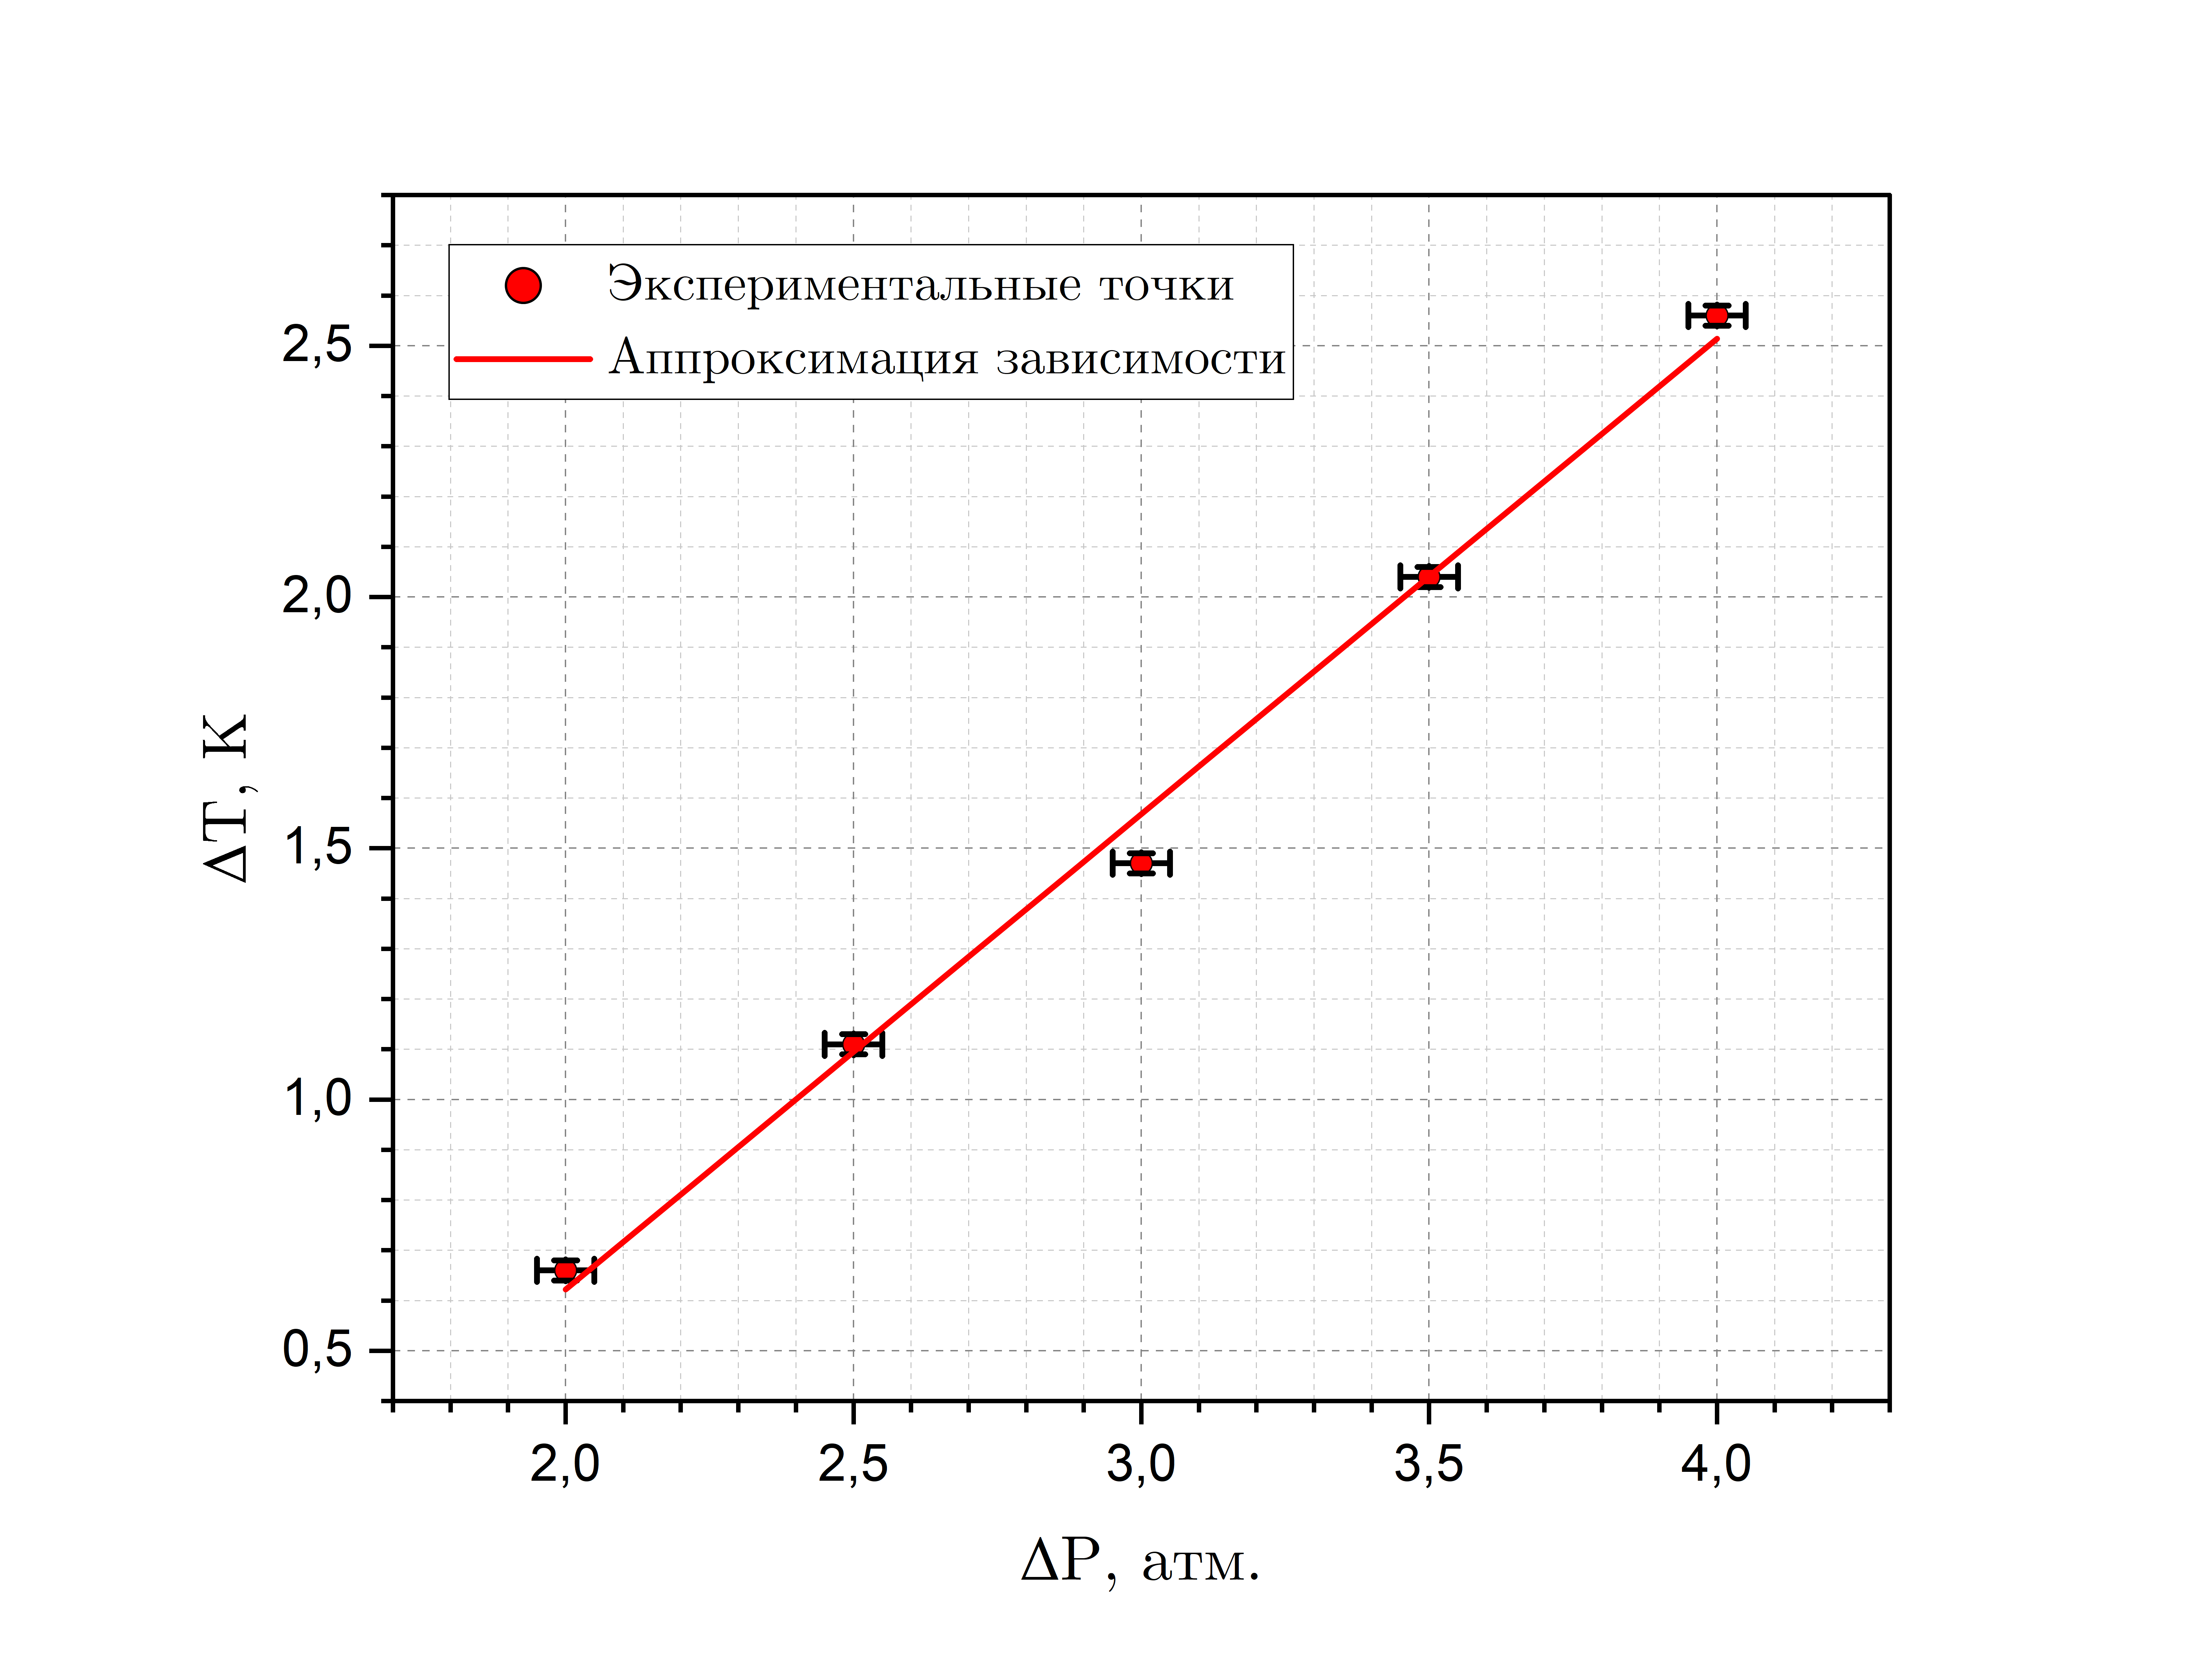
\includegraphics[width=14cm]{images/graph_25.png}
        \caption{График зависимости $\Delta T$ от температуры $\Delta P$ при $T = 25 ^\circ$C}
        \label{graph_25}
    \end{figure}

    \begin{figure}[H]
        \centering
        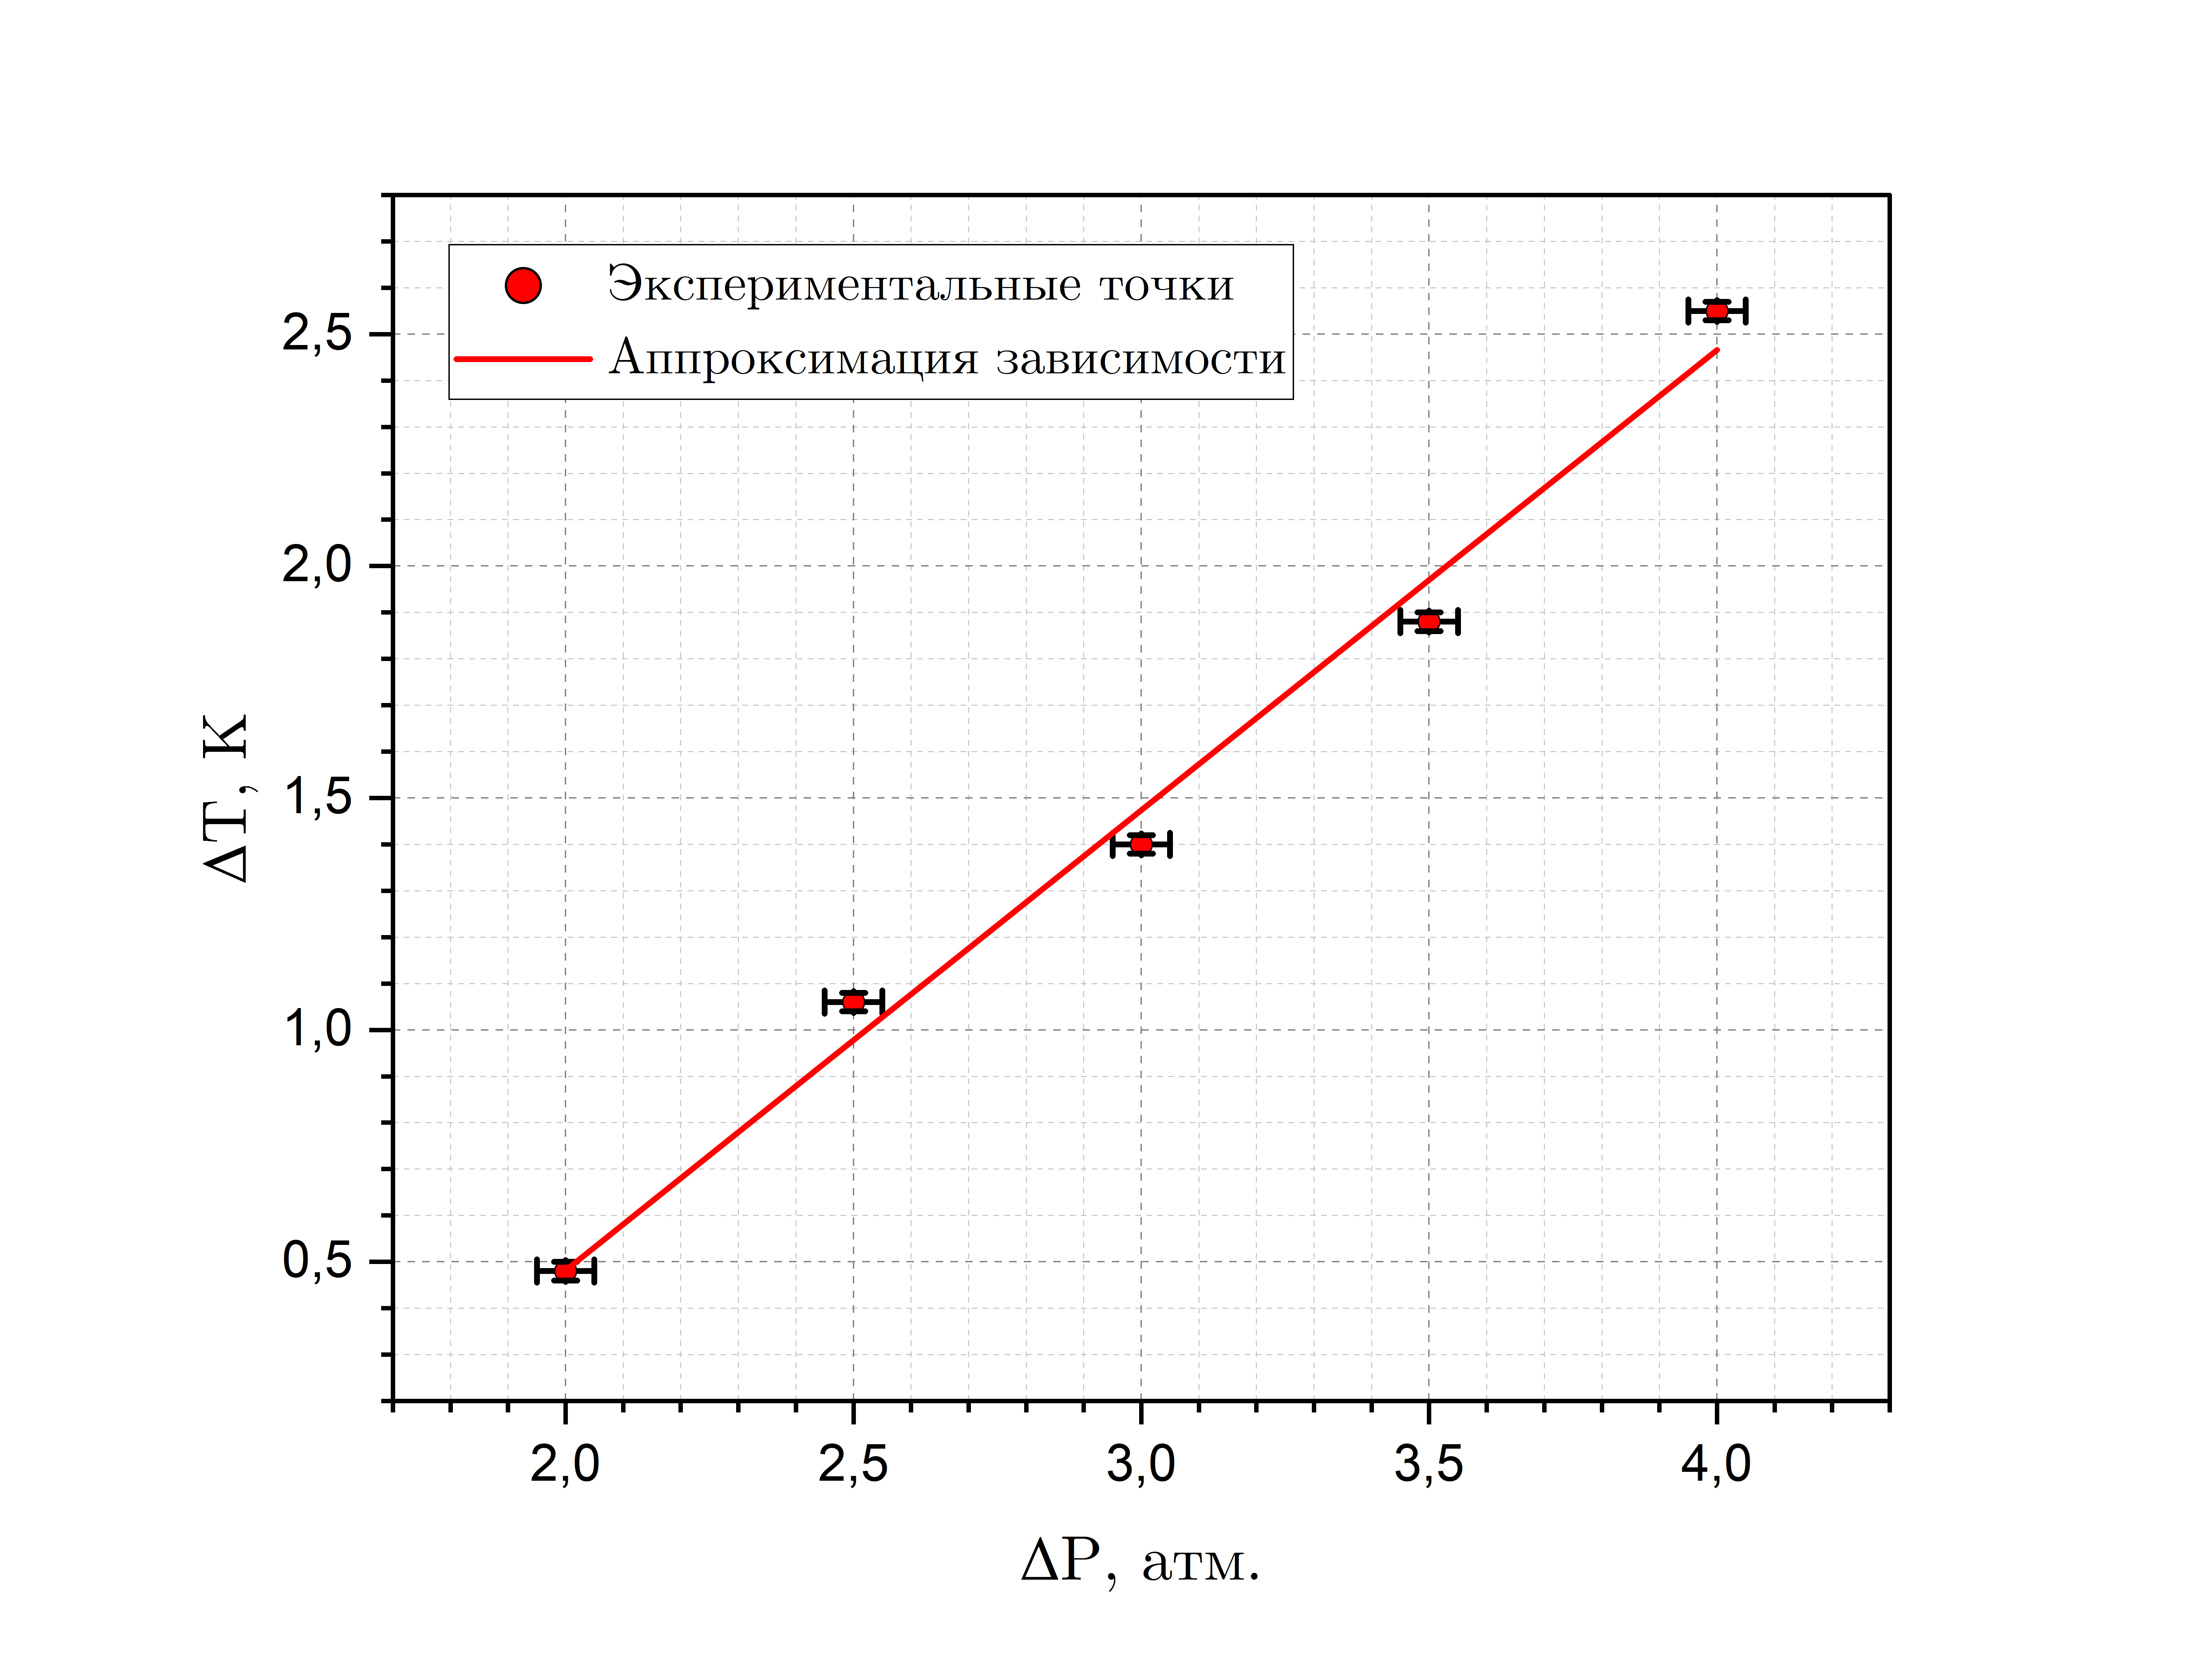
\includegraphics[width=14cm]{images/graph_35.png}
        \caption{График зависимости $\Delta T$ от температуры $\Delta P$ при $T = 35 ^\circ$C}
        \label{graph_35}
    \end{figure}

    \begin{figure}[H]
        \centering
        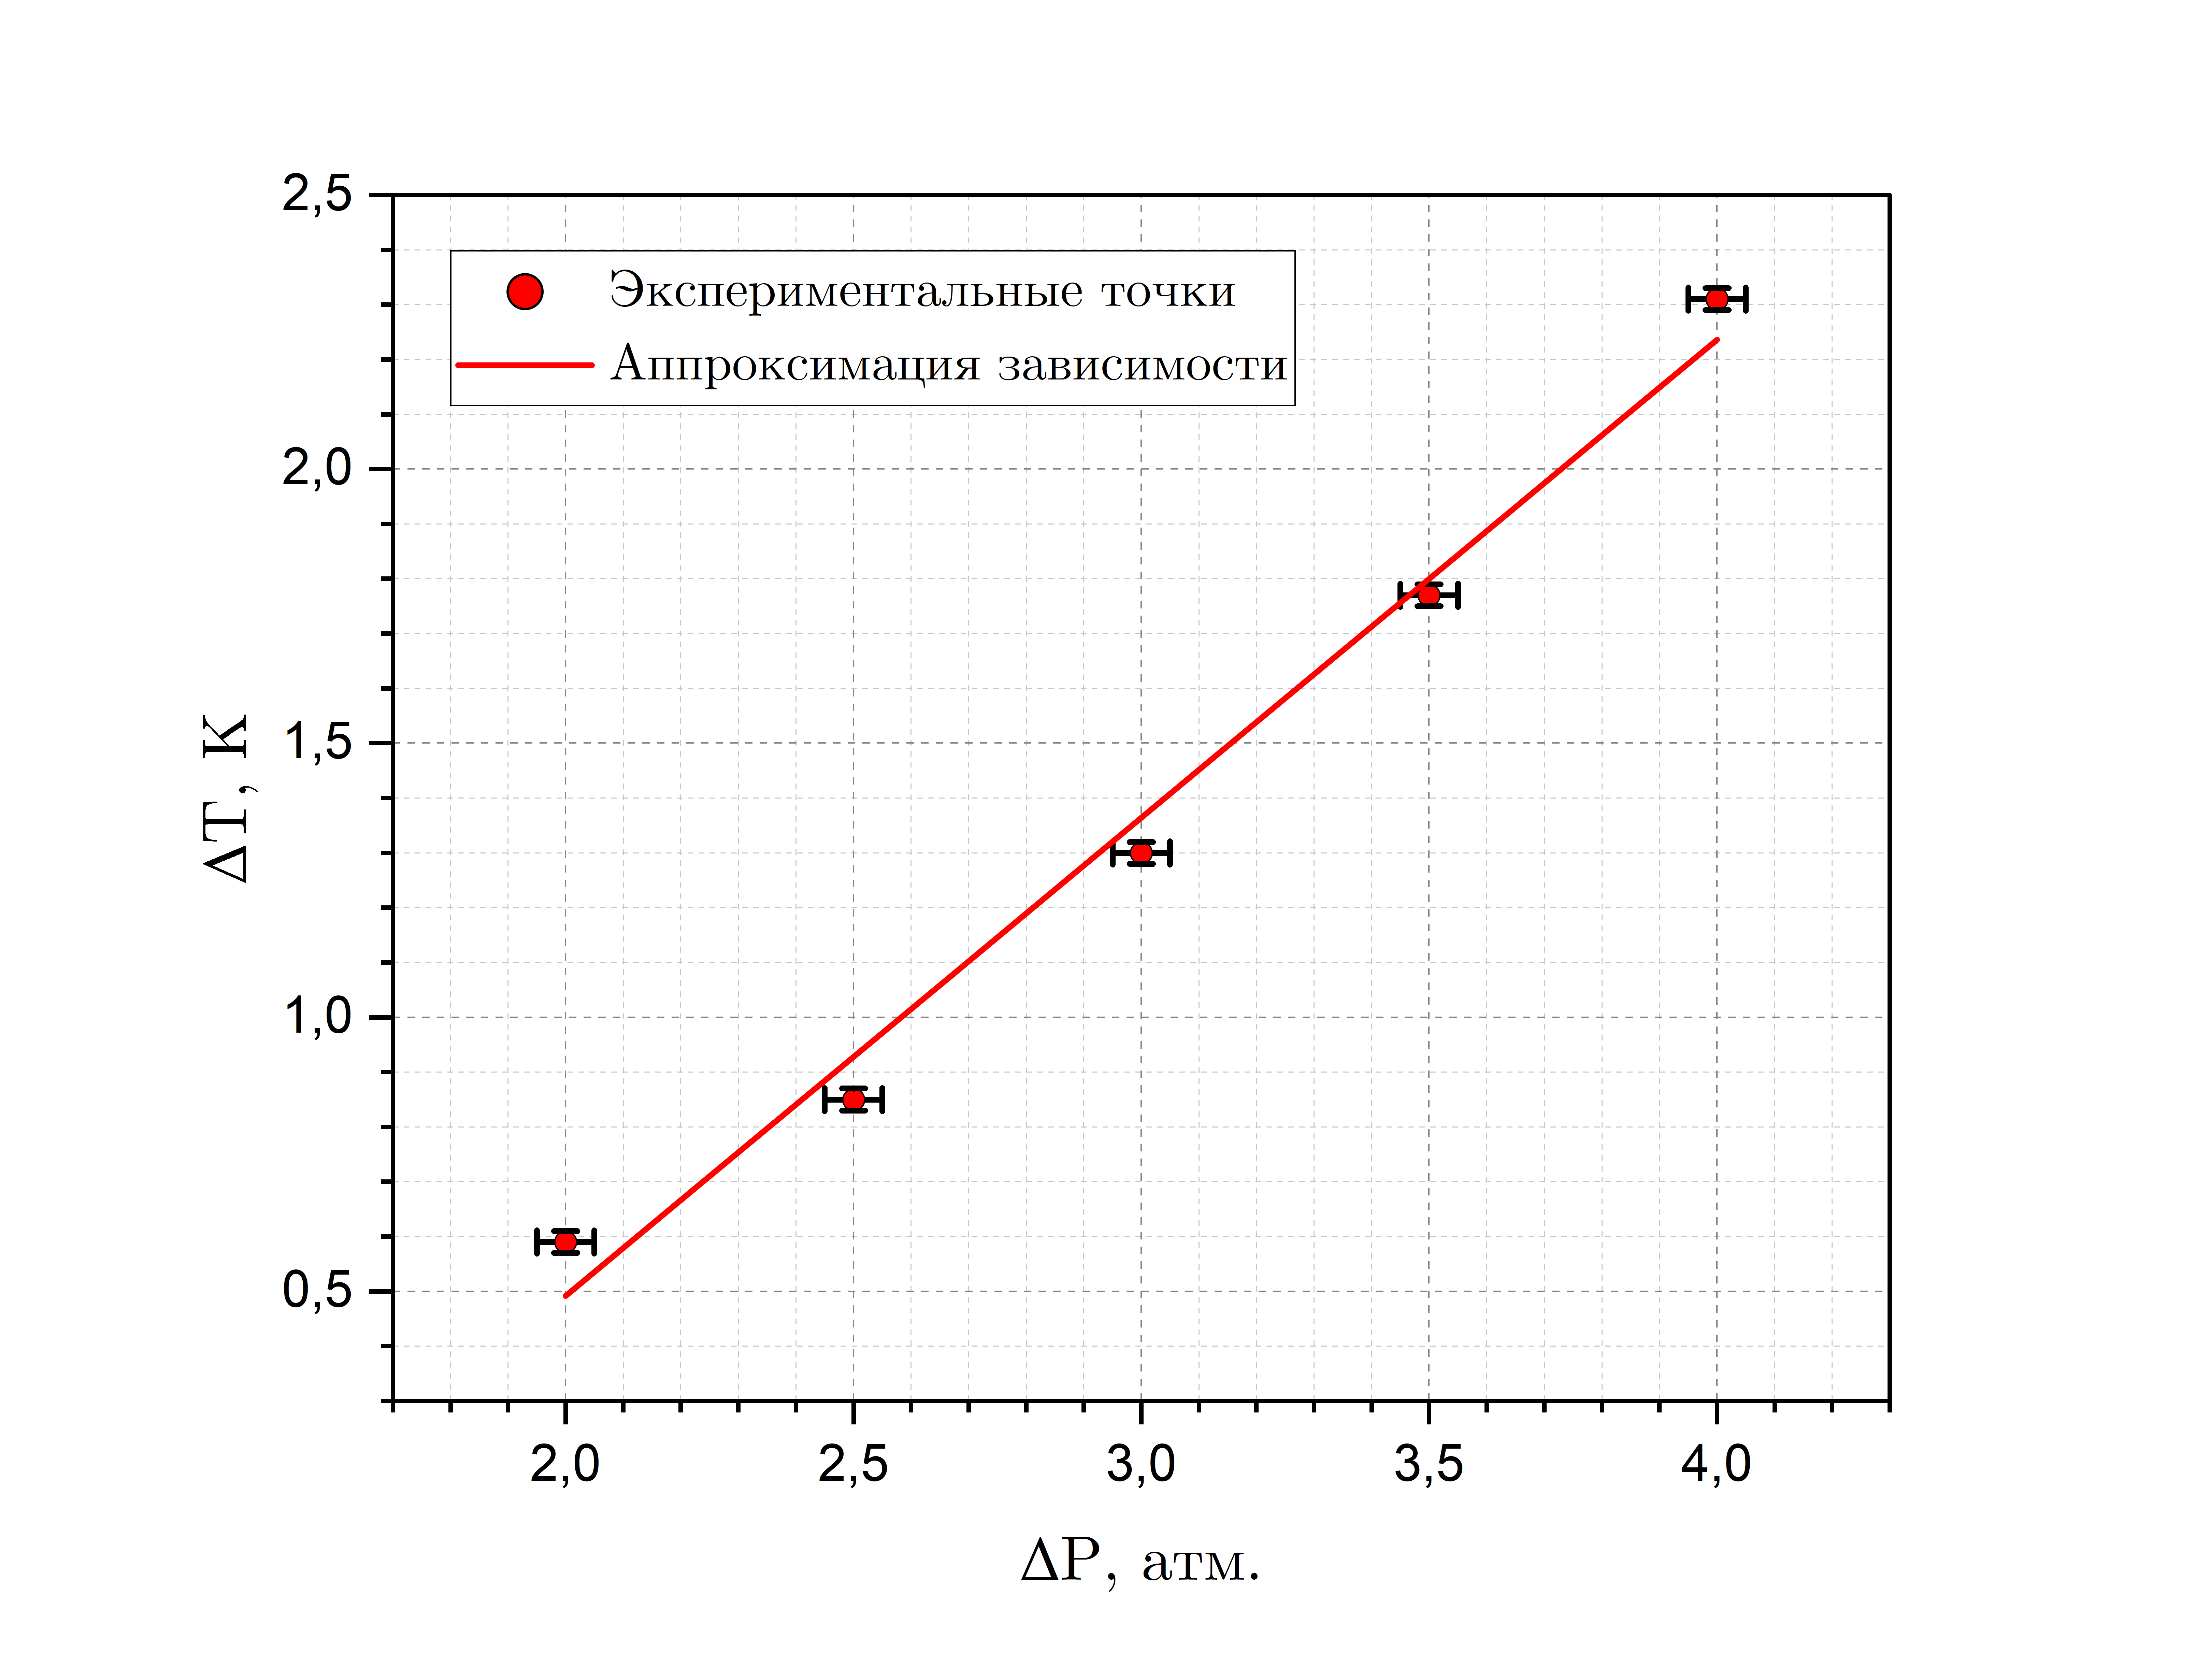
\includegraphics[width=14cm]{images/graph_45.png}
        \caption{График зависимости $\Delta T$ от температуры $\Delta P$ при $T = 45 ^\circ$C}
        \label{graph_45}
    \end{figure}

    \begin{figure}[H]
        \centering
        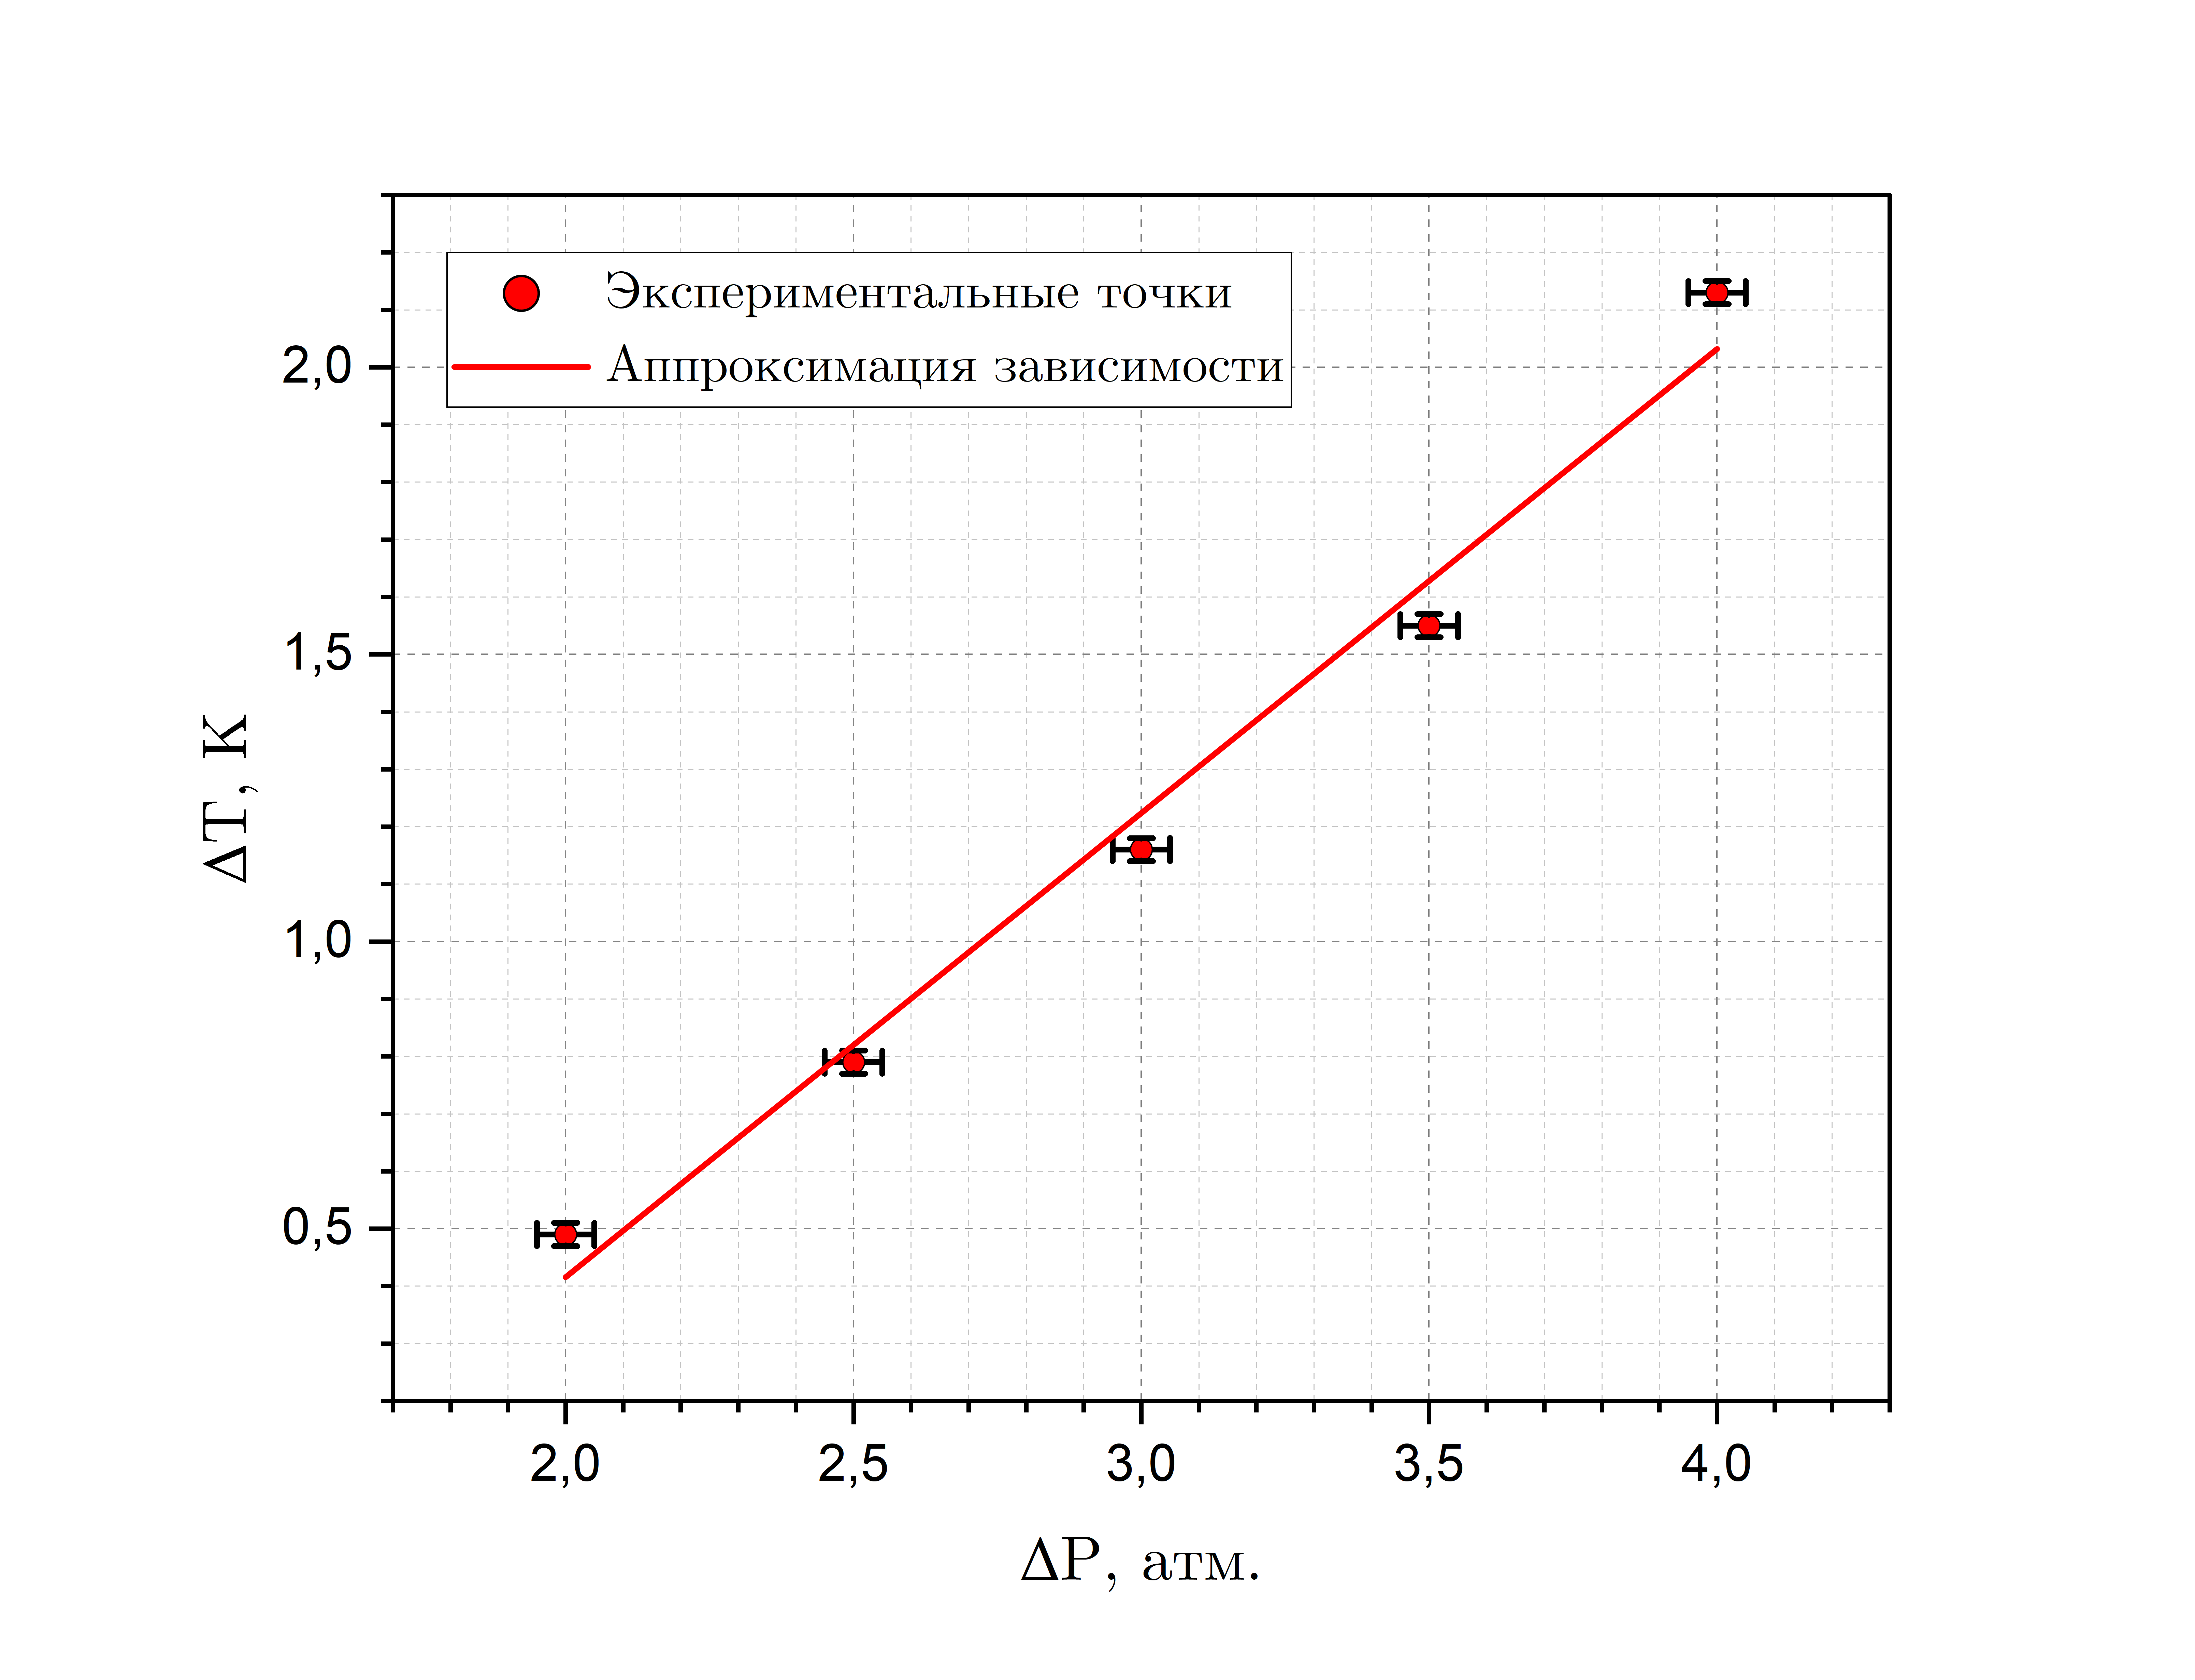
\includegraphics[width=14cm]{images/graph_55.png}
        \caption{График зависимости $\Delta T$ от температуры $\Delta P$ при $T = 55 ^\circ$C}
        \label{graph_55}
    \end{figure}

    \noindent Вычислим $\mu_\text{Д--Т} = \frac{dT}{dP}$, используя метод наименьших квадратов: \[ \mu_\text{Д--Т} = \frac{\langle \Delta P \Delta T \rangle - \langle \Delta P \rangle \langle \Delta T \rangle}{\langle \Delta P \rangle - \langle \Delta P \rangle ^2}.\]

    \noindent Случайную погрешность определения этого коэффициента вычислим по следующей формуле: \[ \sigma^\text{случ}_{\mu_\text{Д--Т}} = \sqrt{\frac{1}{N-2} \left(\frac{\left\langle\left(\Delta T - \langle \Delta T\right\rangle\right)^2 \rangle}{\left\langle\left(\Delta P - \langle \Delta P\right\rangle\right)^2 \rangle}\right)-\mu_\text{Д--Т}^2},\] где  $N$  -- количество измерений.\\

    \noindent Систематические погрешности оценим по следующим формуле: \[ \sigma^\text{сист}_{\mu_\text{Д--Т}} = {\mu_\text{Д--Т}}\sqrt{\varepsilon^2_{\Delta P}+\varepsilon^2_{\Delta T}}.\]
    
    \noindent Таким образом, полная погрешность измерения определяется следующим соотношением: \[ \sigma_{\mu_\text{Д--Т}} = \sqrt{(\sigma_{\mu_\text{Д--Т}}^\text{сист})^2 + (\sigma_{\mu_\text{Д--Т}}^\text{случ})^2}.\]

    \noindent Результаты вычислений заносим в таблицу \ref{tab:my-table}.
    
    \begin{table}[H]
        \centering
        \begin{tabular}{|c|c|c|c|}
            \hline
            $T$, $ ^\circ C $ & $\mu_\text{Д--Т}$, К/атм & $\sigma_{\mu_\text{Д--Т}}$, К/атм & $\varepsilon$, $\%$  \\ \hline
            25 & 0,95 & 0,04 & 4,2 \\ \hline
            35 & 0,99 & 0,06 & 6,0 \\ \hline
            45 & 0,87 & 0,06 & 6,9 \\ \hline
            55 & 0,81 & 0,06 & 7,4 \\ \hline
        \end{tabular}
        \caption{Результаты измерений $ \mu_\text{Д--Т} $}
        \label{tab:my-table}
    \end{table}

    \subsection*{Вычисление параметров газа Ван-дер-Ваальса и температуры инверсии}

    \noindent Построим график зависимости коэффициента Джоуля–Томсона $\mu_\text{Д--Т}$ от обратной температуры $1/T$ (рис. \ref{graph_mu}) с помощью таблицы \ref{tab:ab}.

    \begin{table}[H]
        \centering
        \begin{tabular}{|c|c|c|c|c|}
            \hline
            $t, ^\circ C$ & $T, K$ & $1/T, 10^{-3} \cdot K^{-1}$ & $\mu_\text{Д--Т}$, К/атм & $\sigma_{\mu_\text{Д--Т}}$, К/атм \\ \hline
            25,20 & 298,20 & 3,3535 & 0,95 & 0,04 \\ \hline
            35,06 & 308,06 & 3,2461 & 0,99 & 0,06 \\ \hline
            45,01 & 318,01 & 3,1446 & 0,87 & 0,06 \\ \hline
            55,00 & 328,00 & 3,0488 & 0,81 & 0,06 \\ \hline
        \end{tabular}
        \caption{Зависимость коэффициента Джоуля–Томсона $\mu_\text{Д--Т}$ от обратной температуры $1/T$}
        \label{tab:ab}
    \end{table}

    \noindent Как видно из таблицы, точку, когда температура равна $35 ^\circ C$ нужно отбросить. Коэффициент угла наклона прямой и свободный член найдём, используя метод наименьших квадратов (см. предыдущий пункт).

    $$
    \boxed{\mu_{\text{Д--Т}} = -\left( 0,55 \pm 0,18 \right) \frac{K}{\text{атм}} + \left( 0,45 \pm 0,06 \right) \frac{K}{\text{атм}} \cdot \frac{1000 K}{T}}
    $$

    \noindent Пользуясь формулой \ref{3}, найдём коэффициенты $a$ и $b$:
    \begin{equation}
        \label{eq:a}
        a = \frac{d\mu_\text{Д--Т}}{d(1/T)} \cdot \frac{RC_{p}}{2} = 2R^2 \cdot \left( 450 \pm 6 \right) \frac{K^2}{\text{атм}} = \left( 0,62 \pm 0,01 \right) \frac{\text{Н} \cdot {\text{м}}^4}{{\text{моль}}^2}, \quad a_{\text{табл}} = 0,37 \: \frac{\text{Н} \cdot {\text{м}}^4}{{\text{моль}}^2}
    \end{equation}

    \begin{equation}
        \label{eq:b}
        b = C_p \cdot \left( 0,55 \pm 0,18 \right) \frac{K}{\text{атм}} = \frac{8}{2} R \cdot \left( 0,55 \pm 0,18 \right) \frac{K}{\text{атм}} = \left( 18,3 \pm 6,0 \right) \frac{{\text{см}}^3}{\text{моль}}, \quad b_{\text{табл}} = 42,82 \: \frac{{\text{см}}^3}{\text{моль}}
    \end{equation}

    \begin{figure}[H]
        \centering
        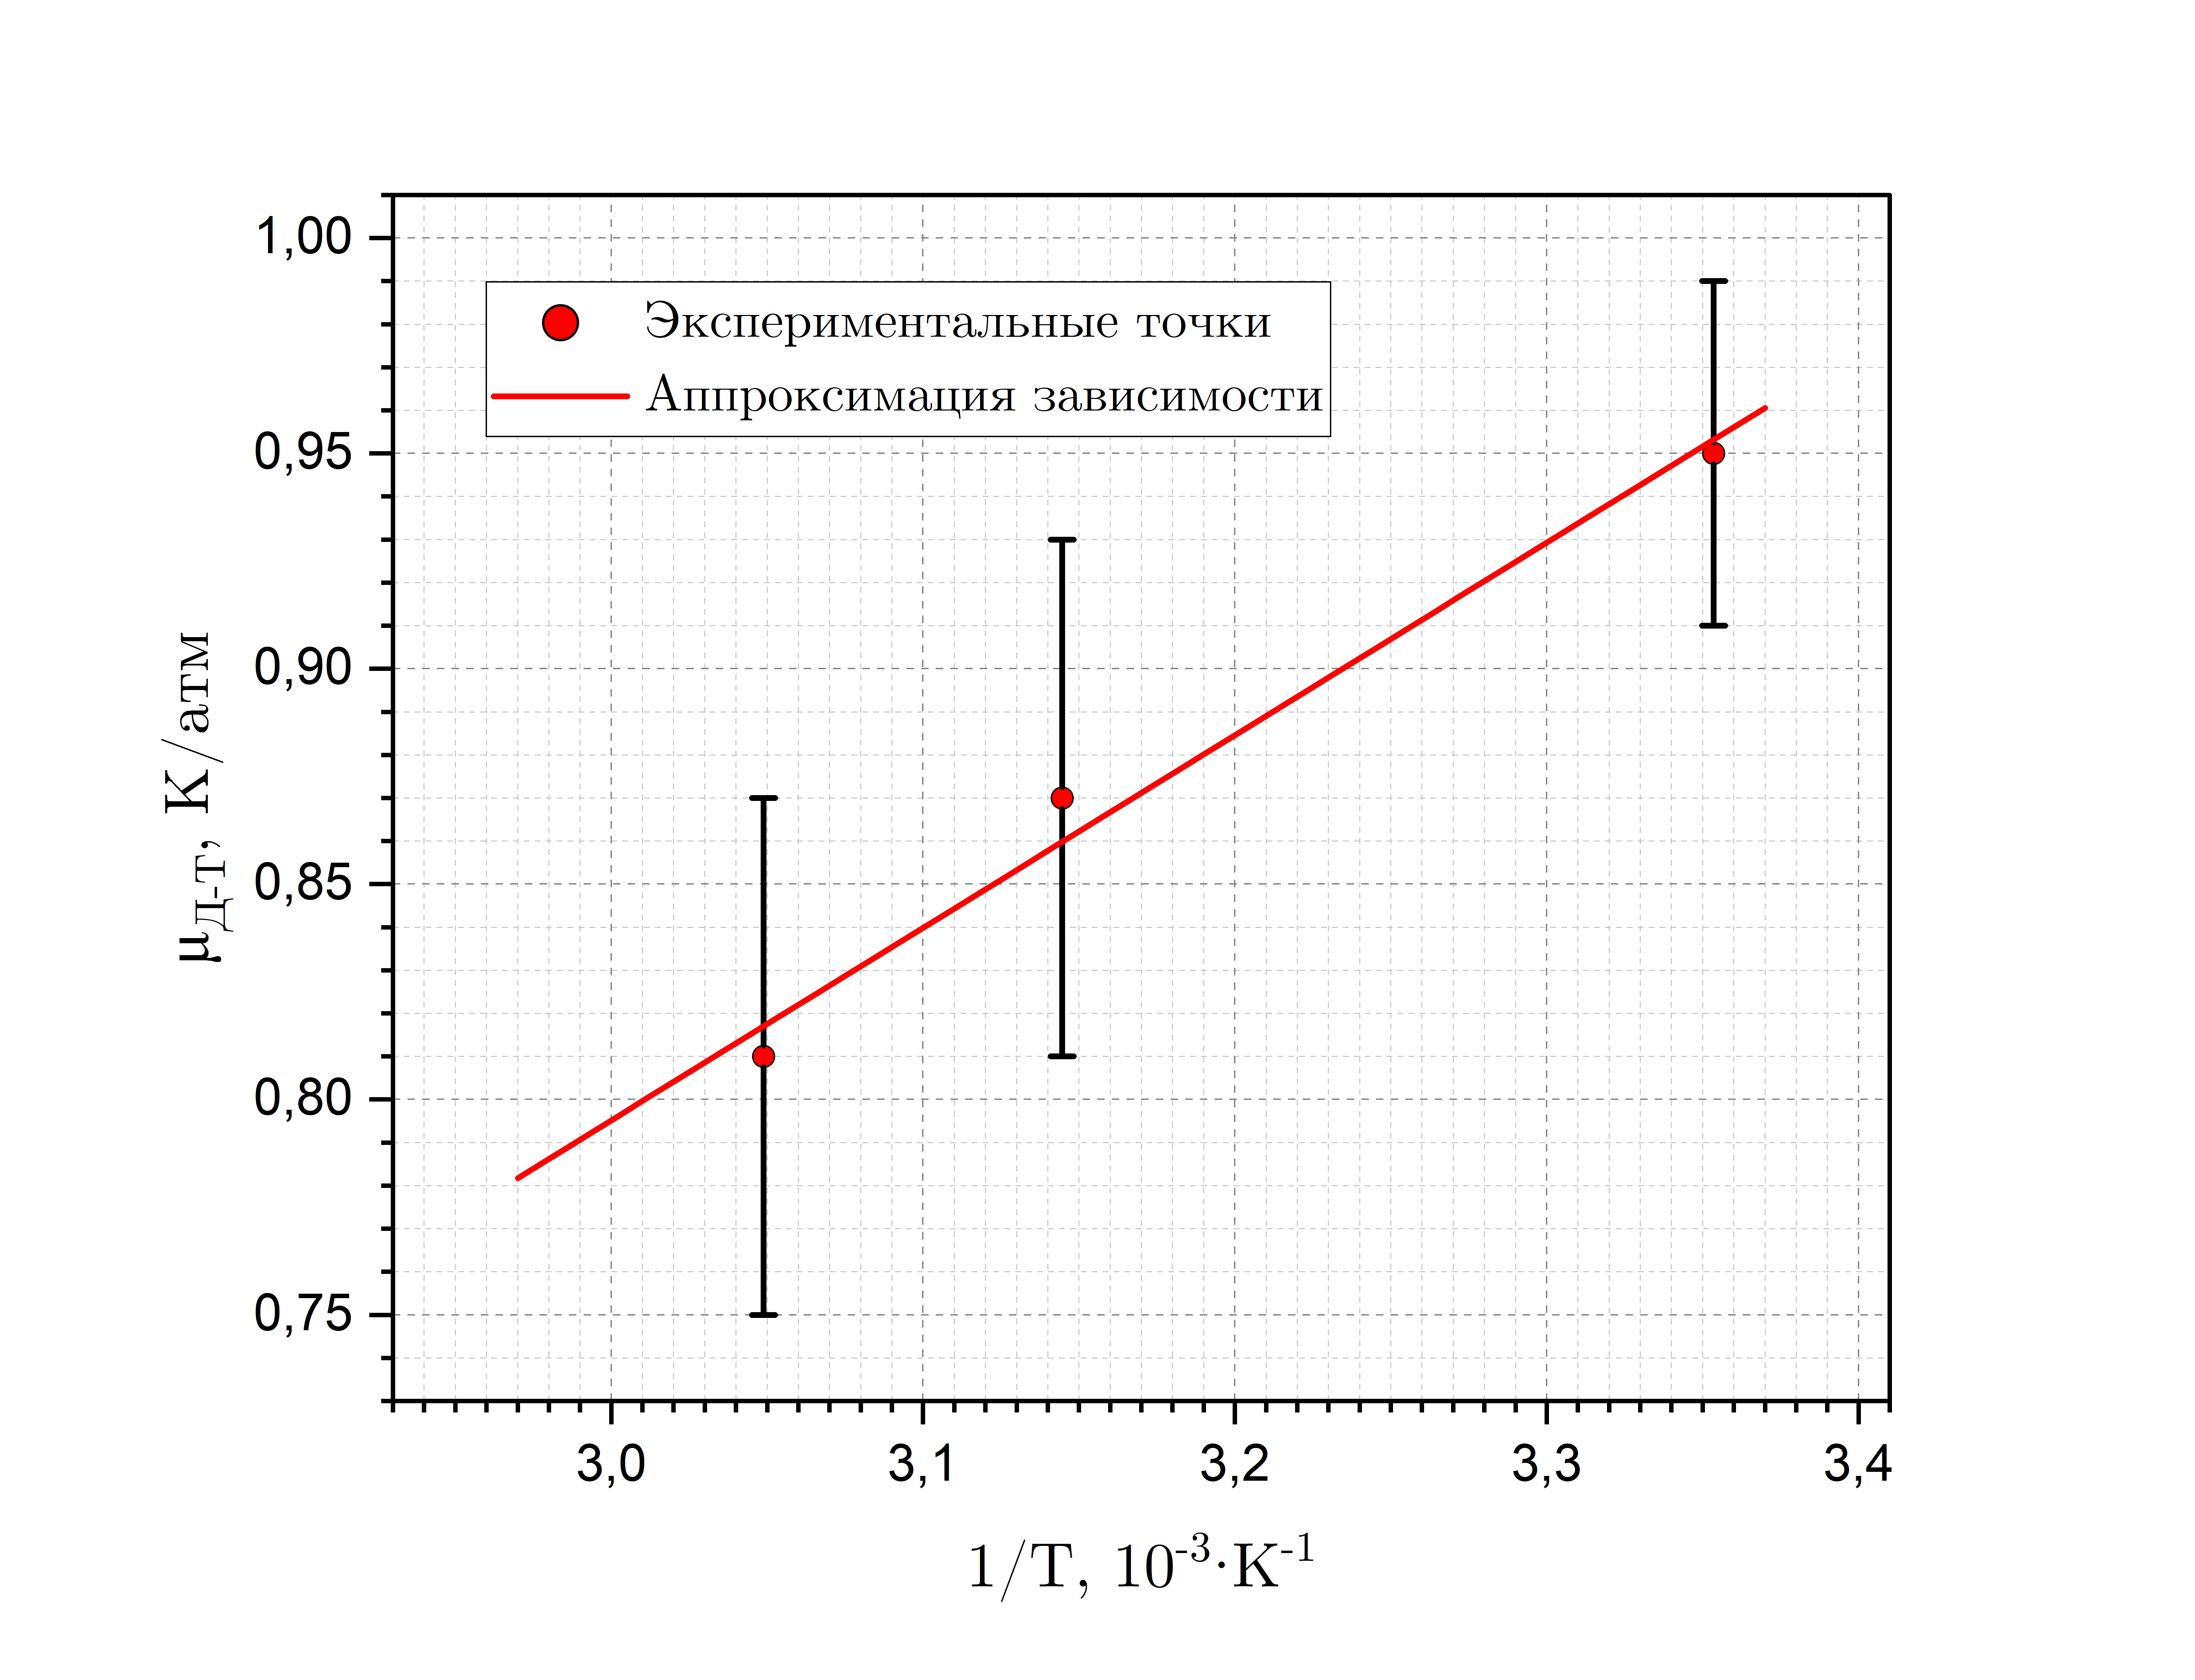
\includegraphics[width=14cm]{images/graph_mu.png}
        \caption{График зависимости коэффициента Джоуля–Томсона $\mu_\text{Д--Т}$ от обратной температуры $1/T$}
        \label{graph_mu}
    \end{figure}

    \noindent Пользуясь соотношениями \ref{eq:a} и \ref{eq:b}, вычислим температуру инверсии:
    \begin{equation}
        T_{\text{инв}} = \frac{2a}{Rb} = 8200 \: K 
    \end{equation}

    \noindent Также рассчитаем погрешность $\sigma_{T_{инв}}$:
    \begin{equation*}
        \sigma_{T_{инв}} = T_{инв}\sqrt{\left( {\varepsilon_a}^2 + {\varepsilon_b}^2 \right)} \approx 2700 \: K
    \end{equation*}

    \noindent Окончательно получим:
    $$
    \boxed{T_{инв} = \left( 8200 \pm 2700 \right) K}
    $$
    
    \section*{Заключение}

    \noindent В ходе выполнения работы:
    \begin{itemize}
        \item вычислили коэффициенты Джоуля-Томсона для разных температур;
        \item экспериментальным методом измерили коэффициенты газа Ван-дер-Ваальса <<a>> и <<b>>;
        \item вычислили $T_\text{инв}$ для углекислого газа.
    \end{itemize}

    \noindent В ходе работы мы получили значения, очень сильно отличающиеся от табличных. Погрешность вычисления параметров газа Ван-дер-Ваальса составила десятки процентов. Такая большая ошибка может говорить нам о неприменимости уравнения Ван-дер-Ваальса в условия лабораторной работы. Действительно, это уравнение используется лишь для качественного описания процессов, происходящих с реальными газами. Количественный подход к этому уравнению не применим.\\

    \noindent Также для увеличения точности измерений можно использовать более точные методы измерения температуры. Повысить точность необходимо как у термостата, так и у вольтметра, т.к. температура на них колебалась на протяжении эксперимента, несмотря на то, что условия оставались неизменными.
    
\end{document}